% ═════════════════════════════════════════════════════════════════════════════
%  Neural MCPF Allocation — final course article
%  Target: 7–10 pages (guideline, not a hard cap), single-column 11pt A4.
%  Structure spec: docs/superpowers/specs/2026-08-10-final-report-structure-design.md
%  Style rules:    report/STYLE.md
%
%  BUILD:  latexmk -pdf final_report.tex
%
%  PLACEHOLDERS: every gap is a red "TODO" box tagged with what is missing
%  (TEXT / TABLE / FIGURE / DATA / COMBINATION). Inline unknowns use \NUM.
%  Search for "TODO" to find them all.
%
%  Spelling: American throughout (see STYLE.md).
% ═════════════════════════════════════════════════════════════════════════════
\documentclass[11pt,a4paper]{article}

% ── Core packages ────────────────────────────────────────────────────────────
\usepackage[margin=1in]{geometry}
\usepackage{graphicx}
\usepackage[table]{xcolor}
\usepackage{colortbl}
\usepackage{booktabs}
\usepackage{tabularx}
\usepackage{float}
\usepackage{enumitem}
\usepackage{amsmath, amssymb}
\usepackage{array}
\usepackage{titlesec}
\usepackage{fancyhdr}
\usepackage{microtype}
\usepackage[colorlinks=true, linkcolor=blue, urlcolor=blue, citecolor=blue]{hyperref}
\usepackage[most]{tcolorbox}
\usepackage{caption}
\captionsetup{font=small, skip=4pt}

\graphicspath{{./}{maps/}{oldmodel_large_nm/}{random_vs_fixed/}{real_maps/}{../presentation/assets/}}

% ── List / float compaction ──────────────────────────────────────────────────
\setlist[itemize]{nosep, leftmargin=*, topsep=2pt, partopsep=0pt}
\setlist[enumerate]{nosep, leftmargin=*, topsep=2pt, partopsep=0pt}
\setlength{\textfloatsep}{10pt plus 2pt minus 2pt}
\setlength{\intextsep}{10pt plus 2pt minus 2pt}
\renewcommand{\topfraction}{0.9}
\renewcommand{\bottomfraction}{0.8}
\renewcommand{\textfraction}{0.08}
\renewcommand{\floatpagefraction}{0.8}

\widowpenalty=10000
\clubpenalty=10000

% ── Colors ───────────────────────────────────────────────────────────────────
\definecolor{primary}{RGB}{31, 73, 125}
\definecolor{accentcol}{RGB}{0, 112, 192}
\definecolor{successbg}{RGB}{209, 231, 221}
\definecolor{successframe}{RGB}{25, 135, 84}
\definecolor{todobg}{RGB}{255, 236, 236}
\definecolor{todoframe}{RGB}{190, 30, 45}

% ── Section headings ─────────────────────────────────────────────────────────
\titleformat{\section}{\large\bfseries\color{primary}}{\thesection}{0.6em}{}[\titlerule]
\titleformat{\subsection}{\normalsize\bfseries\color{accentcol}}{\thesubsection}{0.6em}{}
\titlespacing*{\section}{0pt}{11pt}{4pt}
\titlespacing*{\subsection}{0pt}{8pt}{2pt}

% ── Headers / footers ────────────────────────────────────────────────────────
\pagestyle{fancy}
\fancyhf{}
\lhead{\small\textcolor{gray}{Neural MCPF Allocation}}
\rhead{\small\textcolor{gray}{Multi-Agent Systems, 2026}}
\cfoot{\small\thepage}
\renewcommand{\headrulewidth}{0.4pt}

% ── Callout boxes ────────────────────────────────────────────────────────────
\newtcolorbox{findingbox}[1]{breakable, colback=successbg, colframe=successframe, boxrule=0.9pt,
  arc=1pt, left=7pt, right=7pt, top=4pt, bottom=4pt,
  before upper={\textbf{\color{successframe}#1}\par\smallskip}}

% ── PLACEHOLDER MACHINERY ────────────────────────────────────────────────────
\newtcolorbox{TODO}[1]{breakable, colback=todobg, colframe=todoframe, boxrule=0.9pt,
  arc=1pt, left=7pt, right=7pt, top=4pt, bottom=4pt,
  before upper={\textbf{\color{todoframe}TODO~[#1]}\par\smallskip}}
\newcommand{\NUM}{\textcolor{todoframe}{\textbf{[?]}}}
\newcommand{\TODOin}[1]{\textcolor{todoframe}{\textbf{[TODO: #1]}}}

% ─────────────────────────────────────────────────────────────────────────────
\begin{document}

% ── Title block ──────────────────────────────────────────────────────────────
\begin{center}
{\LARGE\bfseries\color{primary} Neural MCPF Allocation}\\[4pt]
{\large Learning the Goal-Allocation Step of Multi-Agent Path Finding}\\[7pt]
{\normalsize Ofek Yabo \quad\textbar\quad Dayan Badalbaev}\\[2pt]
{\small Multi-Agent Systems, 2026}
\end{center}
\vspace{3pt}
{\color{primary}\hrule height 1.1pt}
\vspace{8pt}

% ── Abstract ─────────────────────────────────────────────────────────────────
\begin{abstract}
\noindent\small
Multi-agent path finding with multiple goals requires deciding which agent visits which goals
before any path can be planned. This allocation sub-problem is a multi-agent traveling salesman
problem, and it is the stage that limits how far the solver can scale. The exact RobustMCPF solver
handles it with an LKH TSP call, then passes a fixed allocation to conflict-based search (CBS) for
collision-free planning, a stage that is comparatively well behaved. We replace only the allocation
step with a learned transformer that is size-agnostic: a single set of weights handles any number of
agents and goals. It reads two shortest-path distance matrices, one from agents to goals and one
between goals, and outputs a distribution over agents for each goal. Since CBS is shared by both
pipelines, any difference in the final plan comes from the allocator alone. We evaluate it at
problem sizes from $2\times2$ up to $50\times100$. Across 28 configurations the collision-free plans
it produces are on average 2\% longer than the solver's optimal plans and at worst 5\% longer, and
every allocation it proposed could be planned without collisions. At paper scale it runs
5.9--9.4$\times$ faster while remaining within
roughly 20\% of optimal. We then ask whether map-specialized allocators beat a single generalist.
Five models, one trained on all four benchmark maps and four trained on a single map each, are
compared on solution quality and wall-time to determine whether map-aware routing is worthwhile.
\TODOin{closing sentence with the headline result, once Exp 16 lands}
\end{abstract}

\vspace{2pt}

% ═════════════════════════════════════════════════════════════════════════════
\section{Introduction}
% ═════════════════════════════════════════════════════════════════════════════

Fleets of autonomous agents such as warehouse robots, delivery drones and search-and-rescue teams
all face the same first decision: given a set of targets and a team of agents, who goes where? The
choice matters. A poor allocation sends agents across each other's paths, inflates total travel,
and creates collisions that a planner then has to resolve. It also has to be made before anything
else, since path planning only becomes meaningful once each agent knows its goals.

Formally this is multi-agent path finding (MAPF) with the added requirement that goals be assigned.
The assignment is not a balanced one-to-one matching. An agent may profitably take zero, one, or
several goals, which makes the structure a multi-agent traveling salesman problem (mTSP). The
RobustMCPF solver~\cite{robustmcpf} solves it exactly in two stages. An LKH TSP call~\cite{lkh}
produces the optimal allocation together with each agent's visit order, and conflict-based search
(CBS)~\cite{cbs} converts that into collision-free paths. The two stages scale very differently.
CBS cost depends on how much the agents interfere with each other, whereas the TSP allocation is
combinatorial in the number of agents and goals, and it is the stage that degrades first as
problems grow.

This work replaces that stage, and only that stage, with a neural network that reads two
breadth-first-search distance matrices: $D$ from agents to goals, and $G$ between goals. Both
pipelines then plan collision-free paths with the same CBS implementation, so the comparison stays
close to like-for-like. The trade is exactness for speed.
A network trained by imitation will not always reproduce the optimum, and the question this report
answers is when accepting that is worthwhile.

\noindent\textbf{Contributions.}
\begin{itemize}
  \item A size-agnostic transformer allocator: one set of weights for any $(N,M)$, with no
        positional embeddings and no padding (Section~\ref{sec:method}).
  \item Evaluation by true CBS execution cost instead of allocation accuracy, which shows that most
        disagreements with the solver are cost-equivalent ties (Section~\ref{sec:setup}).
  \item A design study isolating input representation as the dominant factor, worth more than
        architecture, capacity and data scale combined (Section~\ref{sec:design}).
  \item A characterization of what transfers: map geometry largely does, problem scale does not
        (Section~\ref{sec:design}).
  \item A scale-limit and specialist-versus-generalist study producing a concrete map-routing
        recommendation (Section~\ref{sec:final}).
\end{itemize}

% ═════════════════════════════════════════════════════════════════════════════
\section{Background and Problem Setting}
% ═════════════════════════════════════════════════════════════════════════════

\subsection{Why replace the allocator}

The practical case rests on where the cost sits and how often the problem gets solved. In a
warehouse or a delivery fleet, allocation is re-solved continuously as orders arrive and agents
finish their tasks, and every re-solve pays the combinatorial cost again. An exact allocator is an
excellent choice for a single offline instance and a progressively worse one as throughput
requirements rise. A learned allocator has the opposite profile. Training is expensive and paid
once, while inference is a single forward pass through the network, a fixed sequence of matrix
multiplications with no search involved, whose cost grows far more slowly than the solver's. What is given
up is quality. The report measures that loss in the only unit that matters to a user of the system,
the total number of steps the agents actually walk, counted after collisions have been resolved. It
then identifies where the exchange pays off.

\subsection{Problem formulation}

We work in basic MAPF: a 4-connected grid with static obstacles, deterministic movement, no
orientation and no action delays. An instance consists of $N$ agents at distinct start cells and
$M$ goal cells. Every goal is visited exactly once by exactly one agent, and agents are otherwise
unconstrained. The objective is min-sum, minimizing total path length, subject to the paths being
collision-free.

That freedom is what makes this an mTSP and not an assignment problem. Figure~\ref{fig:bundle}
shows the canonical case of two agents near each other and two distant goals. Splitting the goals
costs 14, while giving both to one agent costs 7. The optimum is unbalanced.

% KNOWN ISSUE, DEFERRED BY DECISION (2026-08-11): the figure labels the bundled tour
% "cost 7" but with its current coordinates (A1 0,0 / A2 1,0 / G1 3,4 / G2 4,4) the true
% cost is 8: A1->G1 = 7, G1->G2 = 1. Split (14) is correct.
% FIX: swap the agents, A1 at (1,0) and A2 at (0,0), in presentation/make_diagrams.py:51.
% Then A1->G1 = 6, A2->G2 = 8, so split = 14 and bundle = 6+1 = 7, both labels true.
% We chose not to regenerate the PNG now. Revisit before submission.
\begin{figure}[htbp]
\centering
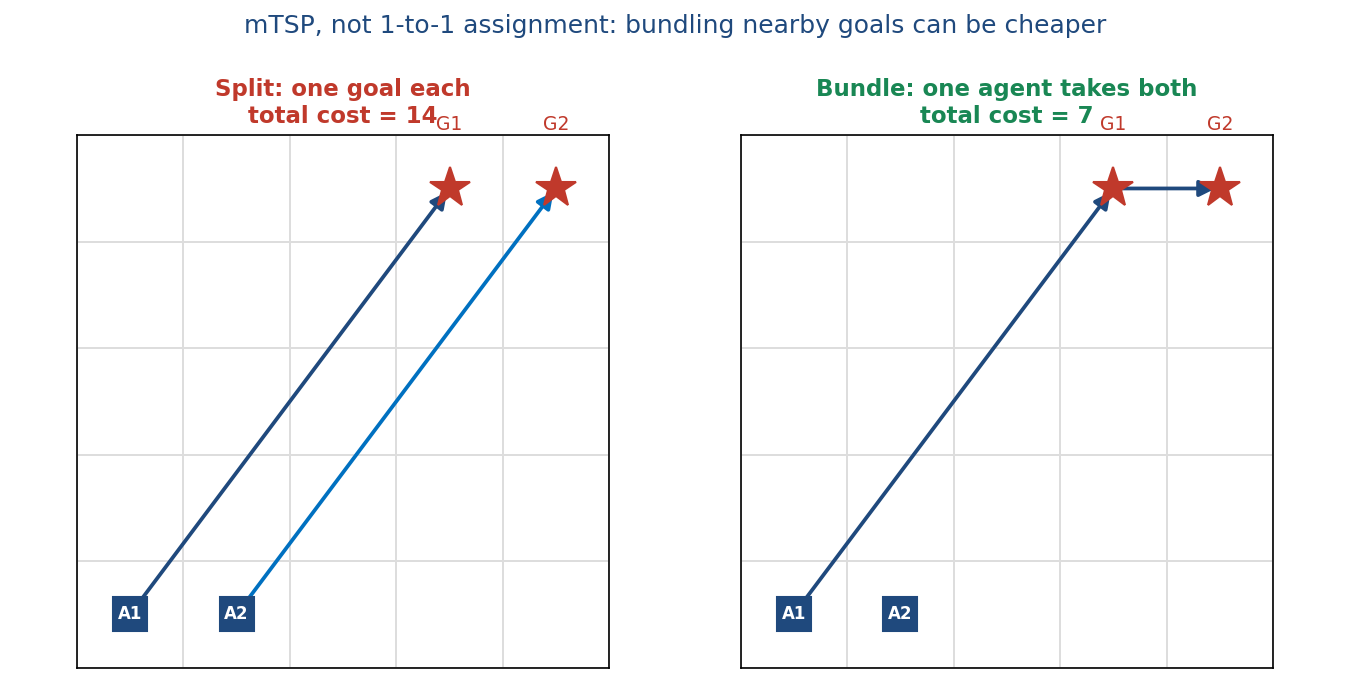
\includegraphics[width=0.58\textwidth]{bundle_vs_split.png}
\caption{Goal allocation is an mTSP, not a balanced assignment. Bundling both goals onto one
agent (cost 7) beats splitting them (cost 14). As a result the ground-truth allocation $Y$ has
columns that sum to one and rows that are free.}
\label{fig:bundle}
\end{figure}

Write $Y \in \{0,1\}^{N \times M}$ with $Y_{ij}=1$ when agent $i$ visits goal $j$. Columns sum to
one and rows are unconstrained. The model therefore has to produce a column-wise distribution,
giving for each goal a distribution over agents, instead of a doubly-stochastic or
permutation-like output. This rules out Sinkhorn-style balanced-assignment layers, which impose a
row constraint the problem does not have.

\subsection{The exact baseline}

RobustMCPF in BasicMAPF mode serves as both ground truth and comparison point. It calls LKH to
solve the underlying TSP, which yields $k$-best allocations along with each agent's visit order,
and then runs CBS to resolve conflicts. We take the cost of the final collision-free plan as the
definitive quality measure. The same solver generates the training labels: every training instance
is solved exactly, and its allocation becomes the supervision target.

\subsection{Related work}

Learning to solve combinatorial problems has a substantial literature. Pointer
Networks~\cite{pointernet} output permutations of their input, reinforcement-learning variants
scaled the idea to routing~\cite{bello}, and attention models became the standard backbone for TSP
and VRP~\cite{kool}; \cite{bengio} surveys the area. Within MAPF, CBS~\cite{cbs} defines the
exact-planning baseline, benchmarks and terminology come from~\cite{stern,sturtevant}, and learned
policies such as PRIMAL~\cite{primal} target path planning, not allocation. Combined target
assignment and planning was formalized by~\cite{ma_koenig}. Closest to our final study is algorithm
selection for MAPF~\cite{kaduri}, which asks the same underlying question of whether
instance-specific specialization beats one general method. We differ from the routing literature in
learning only the allocation and leaving an exact planner downstream, which makes the comparison
end-to-end and unambiguous.

% ═════════════════════════════════════════════════════════════════════════════
\section{Method: The Learned Allocator}
\label{sec:method}
% ═════════════════════════════════════════════════════════════════════════════

\subsection{Overview}

The solver runs LKH followed by CBS. Ours runs a forward pass through the network, then goal-visit
ordering, then CBS (Figure~\ref{fig:pipelines}). Both pipelines plan collision-free paths with the
same CBS implementation. They differ in how the visit order within each agent's goals is obtained:
LKH returns it as part of its tour, whereas our pipeline computes it separately once the allocation
is fixed. For up to eight goals per agent the two agree, since our enumeration is exhaustive and
therefore optimal for a given allocation; Section~\ref{sec:deploy} gives the details. Because the
instance and the cost measure are identical, the difference between the two output plans isolates
the allocation decision.

\begin{figure}[htbp]
\centering
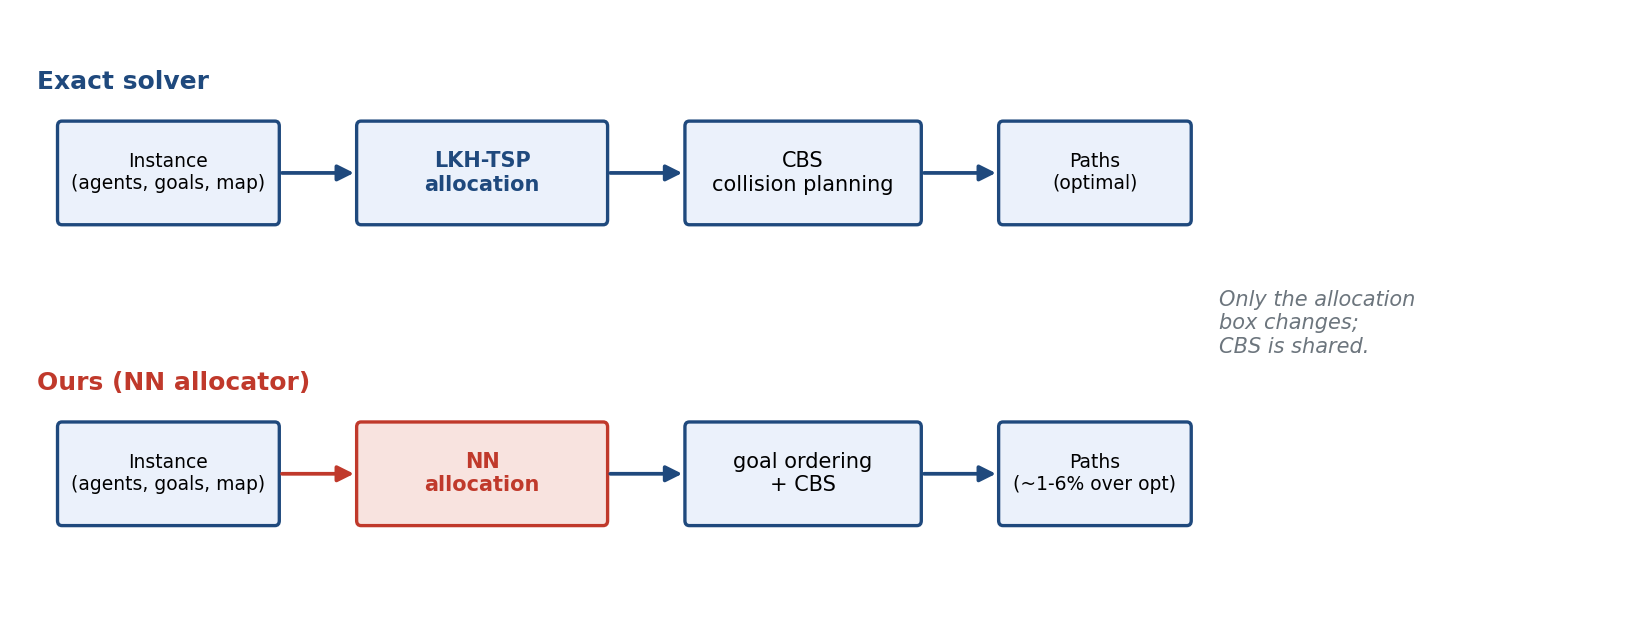
\includegraphics[width=0.86\textwidth]{pipeline_solver_vs_nn.png}
\caption{Only the allocation box changes. CBS is shared, so any difference in execution cost or
wall-time can be attributed to the allocator.}
\label{fig:pipelines}
\end{figure}

\subsection{Input representation}

The network never sees the grid. It sees two matrices of BFS shortest-path distances that respect
walls: $D \in \mathbb{R}^{N \times M}$ from each agent to each goal, and $G \in \mathbb{R}^{M \times
M}$ between goals (Figure~\ref{fig:dg}). Both are divided by $(W-1)+(H-1)$, where $W$ and $H$ are the
grid's width and height in cells. This is the longest shortest path on an open grid of that size,
so it puts distances from grids of different sizes on a common scale. Walls can force a detour that
exceeds it, so it is a scale factor and not a strict bound.

Using distances instead of coordinates is a deliberate choice. Tour cost is a function of
distances, and distances abstract away the map, so the representation transfers across grid sizes
and geometries. $D$ tells each agent how far each goal is. $G$ carries the information $D$ cannot
express, which is which goals lie near each other and should therefore be bundled onto one agent.
Section~\ref{sec:design} shows that $G$ is the single most valuable design decision in the project.

\begin{figure}[H]
\centering
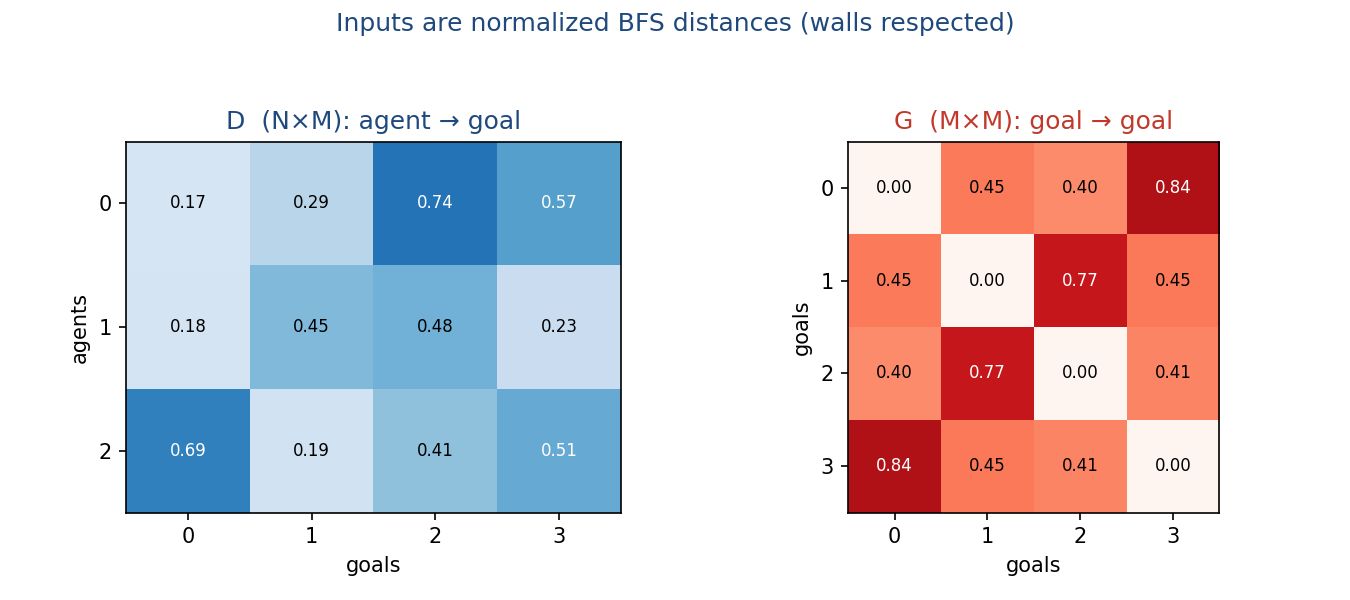
\includegraphics[width=0.54\textwidth]{D_G_matrices.png}
\caption{The two inputs for one instance: agent-to-goal distances $D$ and goal-to-goal distances
$G$, both normalized BFS distances with walls respected.}
\label{fig:dg}
\end{figure}

\subsection{Handling any number of agents and goals}
\label{sec:anynm}

A conventional network fixes its input dimension, which would force one model per $(N,M)$ pair.
Ours does not, and the mechanism is worth setting out in full (Figure~\ref{fig:anynm}).

\textbf{Tokenization.} Each scalar $D_{ij}$ is projected independently to a $d$-dimensional vector
by a shared $\mathrm{Linear}(1 \to d)$, producing an $N \times M$ grid of tokens. Because the
projection is shared, the parameter count does not depend on $N$ or $M$.

\textbf{Goal context.} Goal $j$ has a row of distances to every other goal, $G_{j1}$ through
$G_{jM}$. Each of those numbers is passed through its own shared $\mathrm{Linear}(1 \to d)$, turning
it into a $d$-dimensional vector, and the resulting vectors are then added together elementwise to
give a single $d$-dimensional summary for goal $j$. Embedding before adding matters, because it lets
the network retain more than one property of the distances, and because the sum of any number of
$d$-vectors is still a $d$-vector, $M$ can be anything. That summary is added to each of the $N$
tokens in goal $j$'s column, which are $d$-dimensional as well, so every token concerning goal $j$
also carries information about how that goal sits relative to the rest.

\textbf{Attention.} Each block applies row attention, in which an agent attends over its own goals
and learns how they relate to each other, then column attention, in which a goal attends over the
candidate agents and learns which is best placed to take it, then a feed-forward layer. Blocks are
stacked $L$ deep. Attention operates on variable-length sequences by construction.

\textbf{No positional embeddings.} Agents and goals are unordered sets in an mTSP, so there is no
meaningful ``agent 1''. Leaving out positional embeddings makes the network permutation-equivariant
in both axes and removes the last size-dependent component, which is why the same weights can
process a $2\times2$ instance and a $50\times100$ one.

The architecture therefore places no upper bound on $N$ or $M$. The largest instances reported here,
50 agents and 100 goals, are limited by the exact solver instead: every result is a ratio against its
output, so the baseline has to finish before a comparison exists at all. Section~\ref{sec:final}
measures where that ceiling actually falls.
\TODOin{update the $50\times100$ figure here and in the abstract if the Exp 16 scale sweep pushes past it}

\textbf{Output.} A shared $\mathrm{Linear}(d \to 1)$ reduces each token to a single logit, giving an
$N\times M$ logit matrix. A softmax down each column yields $P$, where $P_{ij}$ is the probability
that agent $i$ visits goal $j$ and $\sum_i P_{ij}=1$. This is exactly the structure
Section~2.2 requires. Taking the arg-max of each column decodes the binary allocation.

\textbf{Mixed-size training.} Instances of different shapes cannot be stacked into one rectangular
array, which is what a GPU needs in order to process many at once, so a
\texttt{MixedSizeBatchSampler} builds shape-homogeneous batches. Each batch holds a single $(N,M)$
while consecutive batches differ, which trains one model jointly across many configurations without
padding or masking.

\begin{figure}[htbp]
\centering
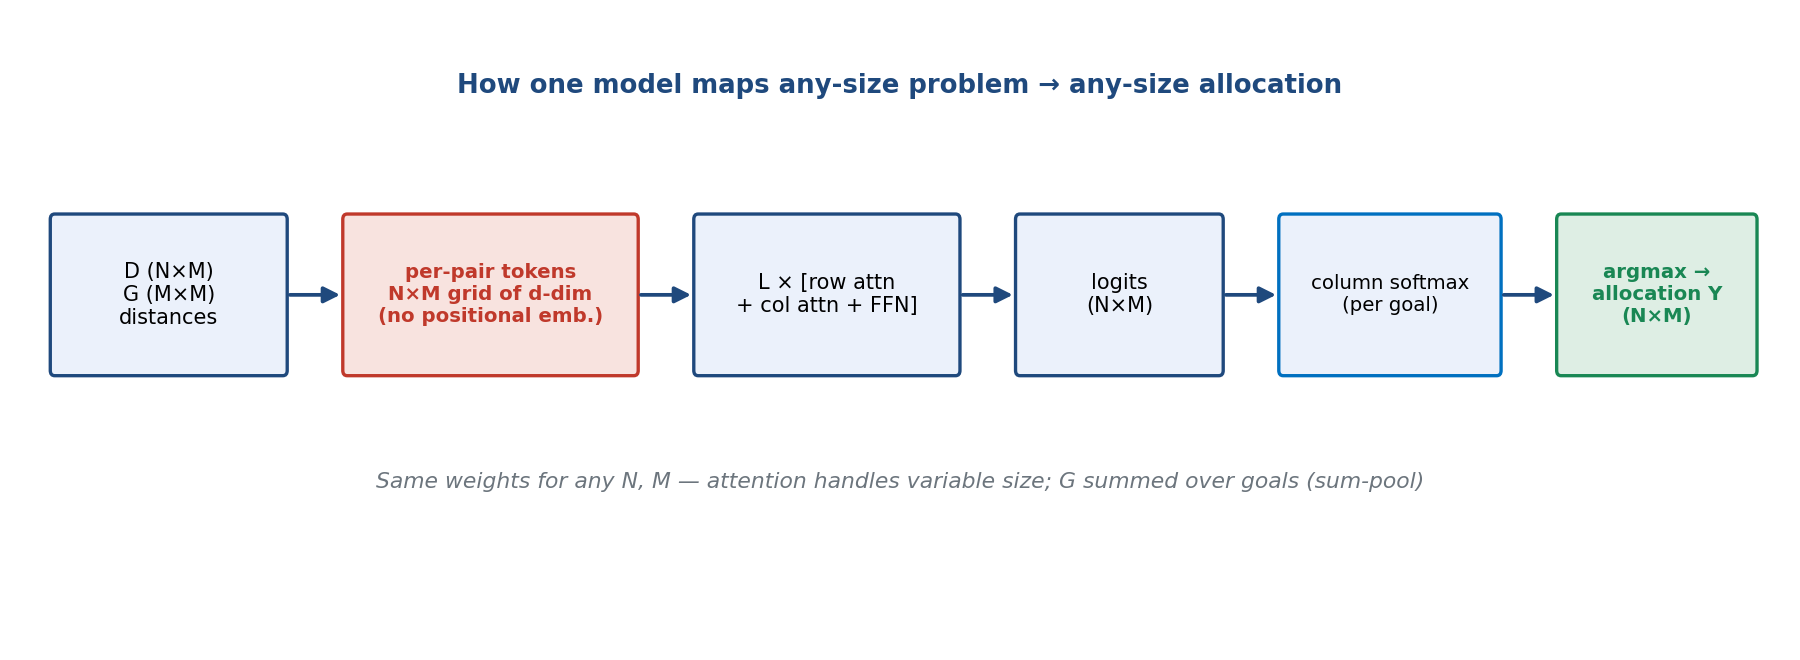
\includegraphics[width=0.96\textwidth]{anyNM_pipeline.png}
\caption{The size-agnostic path from an instance to an allocation. $D$ and $G$ become an $N\times M$
token grid, row/column attention blocks process it, a shared head produces $N\times M$ logits, a
column softmax gives a per-goal distribution over agents, and arg-max decodes the allocation. No
stage depends on the values of $N$ or $M$.}
\label{fig:anynm}
\end{figure}

\subsection{Loss}

Training minimizes
\[
\mathcal{L} = \mathcal{L}_{\mathrm{CE}} + \lambda\,\mathcal{L}_{\mathrm{MinSum}},
\qquad
\mathcal{L}_{\mathrm{CE}} = -\tfrac{1}{M}\textstyle\sum_{j}\sum_{i} Y_{ij}\log P_{ij},
\qquad
\mathcal{L}_{\mathrm{MinSum}} = \tfrac{1}{M}\textstyle\sum_{i,j} P_{ij} D_{ij},
\]
with $\lambda = 0.1$. The cross-entropy term is per-goal imitation of the solver and does most of
the work. The min-sum term is a mild geometric regularizer that penalizes assigning distant goals
and prevents degenerate near-uniform predictions early in training. It is only a first-hop proxy,
with no tour chaining and no collision term, so the true mTSP objective reaches training solely
through the labels $Y$.

\subsection{Data generation and deployment}
\label{sec:deploy}

Each sample is produced by placing agents and goals on a map, computing $D$ and $G$ by BFS, and
calling the solver for the optimal $Y$. Instances with unreachable goals are rejected, as are those
that exceed a CBS node budget of 50k expansions. That second filter addresses a failure mode found
at high wall density, where an instance passes the reachability check but CBS escalates constraints
without ever terminating.

At deployment the arg-max allocation is decoded, each agent's visit order is fixed, and CBS plans
the paths. Ordering is done by exhaustive enumeration: for an agent holding $k$ goals we evaluate
all $k!$ orderings and keep the cheapest, which is optimal by construction. Beyond eight goals per
agent the enumeration becomes impractical, so we fall back to nearest-neighbor construction followed
by 2-opt improvement. When an allocation admits no
collision-free plan, the next candidate in a probability-ranked chain is tried, taken best-first
over the joint probability $\prod_j P_{a_j,j}$ up to $k=3$. This is the learned counterpart of the
solver's $k$-best escape.

% ═════════════════════════════════════════════════════════════════════════════
\section{Experimental Setup and Metrics}
\label{sec:setup}
% ═════════════════════════════════════════════════════════════════════════════

Experiments run on procedurally generated grids and on the four $32\times32$ benchmark maps that
RobustMCPF itself uses (Figure~\ref{fig:maps}). Only \texttt{maze} and \texttt{room} have genuine
corridor and room structure, while \texttt{empty} and \texttt{random} are unstructured. That
distinction drives several of the results below.

\begin{figure}[htbp]
\centering
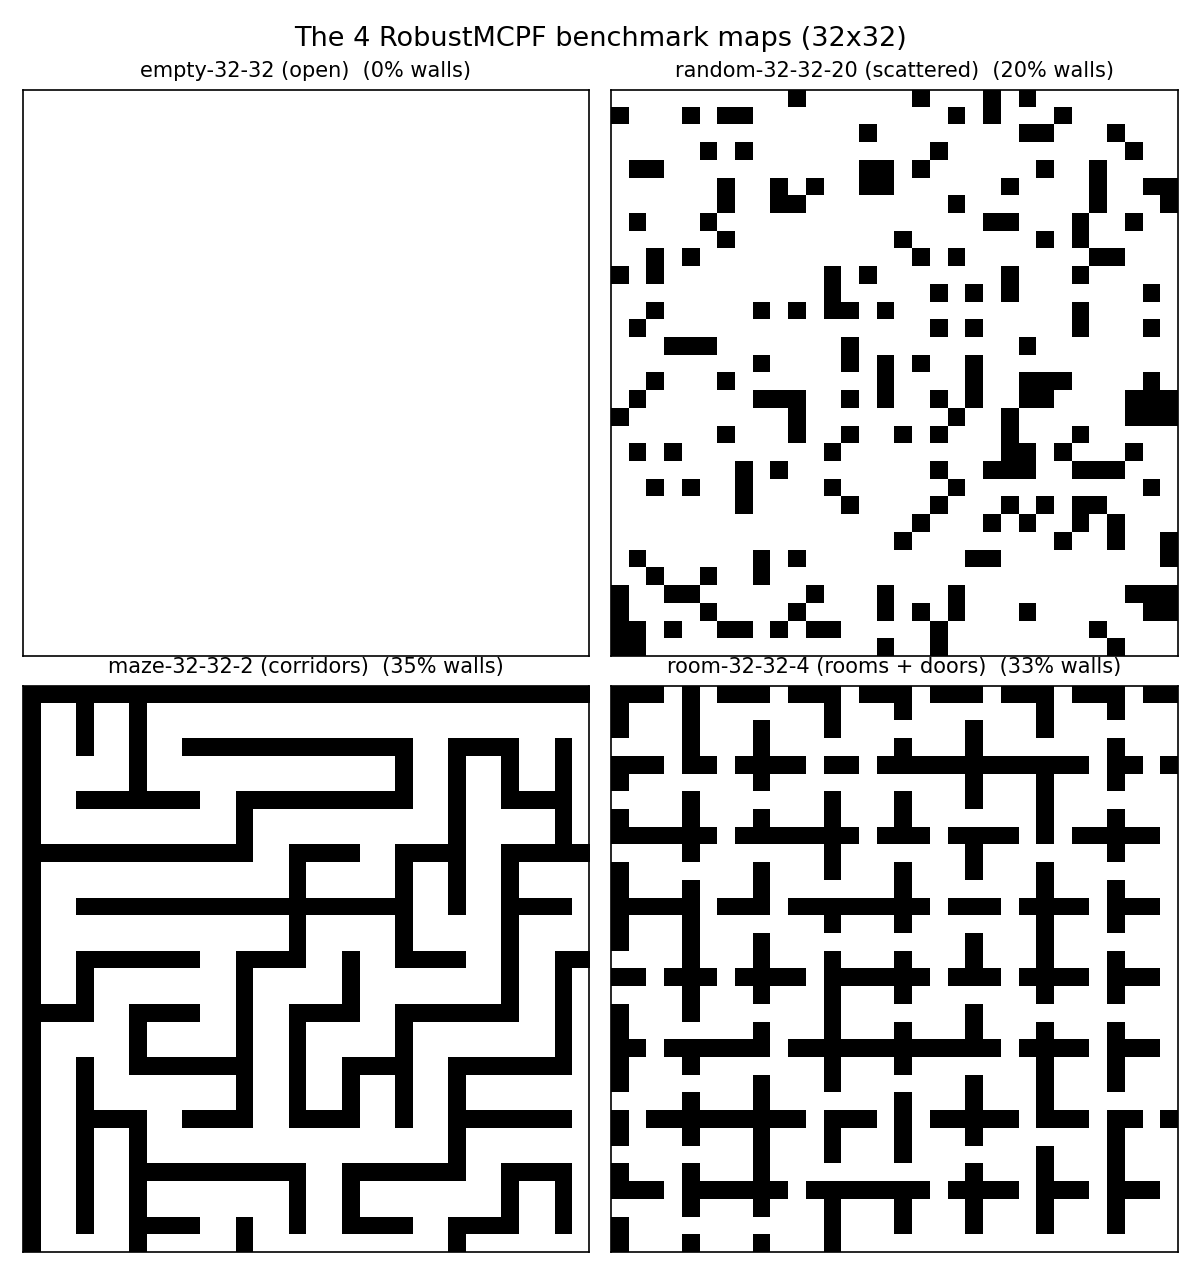
\includegraphics[width=0.46\textwidth]{maps_panel.png}
\caption{The four $32\times32$ benchmark maps: \texttt{empty}, \texttt{random-32-32-20},
\texttt{maze-32-32-2} and \texttt{room-32-32-4}. Only the last two are structured.}
\label{fig:maps}
\end{figure}

\textbf{Allocation-quality metrics} compare predicted and ground-truth allocations directly, with
no planning involved. Per-goal accuracy is the fraction of goals routed to the solver's chosen
agent. It is a lenient measure, since one wrong goal out of $M$ still scores $(M{-}1)/M$.
Full-assignment accuracy is the all-or-nothing indicator that every column matches, and it
empirically tracks (per-goal accuracy)$^{M}$. A proxy cost ratio compares only the first-hop BFS
cost of the two allocations. Because it ignores tour chaining and collisions, values below $1.0$
reflect the metric's mismatch with the true objective and not the network beating the solver.

\textbf{Execution-cost metrics} run both pipelines end to end, where a plan's cost is the total
collision-free path length in grid steps that CBS returns. Cost ratio is the per-instance
$c_{\mathrm{nn}}/c_{\mathrm{sol}}$ averaged over instances, so $1.0$ means the network matched the
exact solver. Exact match is the fraction of instances whose two integer costs are identical, and
it runs far higher than full-assignment accuracy because many distinct allocations are
cost-equivalent ties. Diff is the mean gap in grid steps, speedup is the ratio of mean
single-instance wall-times on the same node, and the infeasible and fallback counters report how
often the candidate chain was needed. These are the numbers that matter, because they measure the
plan an agent would actually execute.

% ═════════════════════════════════════════════════════════════════════════════
\section{Design Study: What Shaped the System}
\label{sec:design}
% ═════════════════════════════════════════════════════════════════════════════

Fifteen experiments preceded the final system. Instead of recounting them chronologically, we
report the five findings that determined the design, each of which fixes one property described in
Section~\ref{sec:method}. Table~\ref{tab:decisions} collects the supporting numbers. Throughout this
section $N$ is the number of agents and $M$ the number of goals, and differences in accuracy are
quoted in percentage points: a model scoring 0.789 against one scoring 0.772 is ahead by 1.7 points.

\textbf{D1. Attention wins, and increasingly so with scale.} Against an MLP and a DeepSets encoder
on identical data, the row/column transformer led on every metric, and its margin over the MLP grew
from $1.7$ points of full-assignment accuracy at $N{=}2$ to $6.7$ points at $N{=}5$. Cross-goal
interdependence is what widens as problems grow, and attention is what captures it. This fixes the
backbone.

\textbf{D2. Representation dominates everything else.} Adding $G$ lifted full-assignment accuracy
by 14 to 18 points at every agent count. For comparison, doubling the training set from 10k to 20k
samples bought $0.4$ points, and every capacity increase we tried bought at most $1.4$, with the
largest configuration diverging outright. $D$ on its own cannot express the fact that two goals are
adjacent and should be bundled. $G$ supplies precisely that, and it is worth more than architecture,
data and capacity put together: about four times as much at $N{=}2$ and roughly twice as much at
$N{=}5$. This fixes the input.

\textbf{D3. One size-agnostic model beats a family of specialists.} A universal model trained
jointly across fifteen $(N,M)$ configurations matched or beat the per-size specialists on all but
the easiest configuration, gaining $2.4$ to $3.5$ points. It also transferred upward. Evaluated on
$N{=}5$, which it had never seen in training, it beat the specialist trained on $N{=}5$ by $3.5$
points. Cross-configuration training acts as a regularizer and pushes the model toward the
allocation principle instead of size-specific patterns. This justifies the universal architecture.

\textbf{D4. Allocation accuracy is the wrong yardstick.} Measured end to end, the fraction of
instances whose plan costs exactly what the solver's costs (64--97\%) far exceeds the fraction on
which the same allocation is chosen (44--91\%). Many disagreements are ties, with two agents
equidistant from a goal and either choice equally good, so a model judged on allocation accuracy
alone looks considerably worse than it performs. This is why every headline number in this report
is an execution cost.

\textbf{D5. Geometry transfers, scale does not.} A model trained only on small random grids and
evaluated zero-shot on the four real maps at small $N,M$ reached a cost ratio of $1.019$, meaning no
meaningful degradation. Structured maps even proved easier than open ones, because walls remove the
ties that an open grid leaves to chance. Pushed to large $N,M$, the same model collapsed to $1.246$
against a map-trained model's $1.048$, with a revealing signature: at $M{=}30$, adding agents hurt
the model trained on $N\le5$ while helping the in-range model (Figure~\ref{fig:designfigs}b).
Separately, training on cheap random grids matched training on the real maps everywhere except the
maze, where random obstacles never reproduce corridor structure. This is why the final models are
retrained at the target scale and on the target maps, and it is the direct motivation for
Section~\ref{sec:final}.

\begin{table}[htbp]
\centering
\caption{Design decisions and the evidence behind them. Effects are on full-assignment accuracy
(D1--D3) or execution-cost ratio (D4--D5).}
\small
\begin{tabularx}{\textwidth}{llX}
\toprule
\textbf{Decision} & \textbf{Effect} & \textbf{Evidence} \\
\midrule
Transformer backbone            & $+1.7 \to +6.7$ pt   & vs.\ MLP, margin growing over $N{=}2\ldots5$ \\
\textbf{Add goal-goal distances $G$} & $\mathbf{+14.2 \to +18.0}$ \textbf{pt} & with vs.\ without $G$, all agent counts \\
More data (10k $\to$ 20k)       & $+0.4$ pt            & gains already flattening at 20k \\
More capacity (to h256/L6)      & $\le +1.4$ pt        & largest configuration diverges at lr $10^{-3}$ \\
Size-agnostic universal model   & $+2.4 \to +3.5$ pt   & vs.\ per-size specialists; $+3.5$ pt zero-shot at $N{=}5$ \\
Judge by CBS execution cost     & 64--97\% vs.\ 44--91\% & exact-cost match vs.\ exact-allocation match \\
Train on the target map family  & $1.048$ vs.\ $1.075$ & fixed-map vs.\ random; the gap is entirely the maze ($1.029$ vs.\ $1.127$) \\
Retrain at the target scale     & $1.048$ vs.\ $1.246$ & map-trained vs.\ small-scale model at large $N,M$ \\
Smaller network in-distribution & $1.048$ vs.\ $1.052$ & h128/L6 vs.\ h256/L8; $2.5\times$ the parameters bought nothing \\
\bottomrule
\end{tabularx}
\label{tab:decisions}
\end{table}

\begin{figure}[htbp]
\centering
\begin{minipage}[b]{0.475\textwidth}
  \centering
  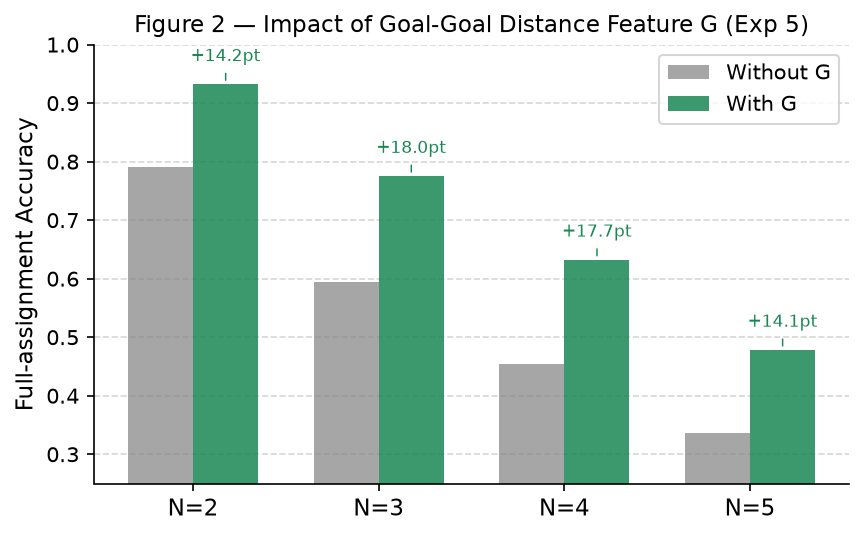
\includegraphics[width=\textwidth]{fig2_ablation.png}\\[1pt]
  {\small (a) the $G$ ablation}
\end{minipage}\hfill
\begin{minipage}[b]{0.475\textwidth}
  \centering
  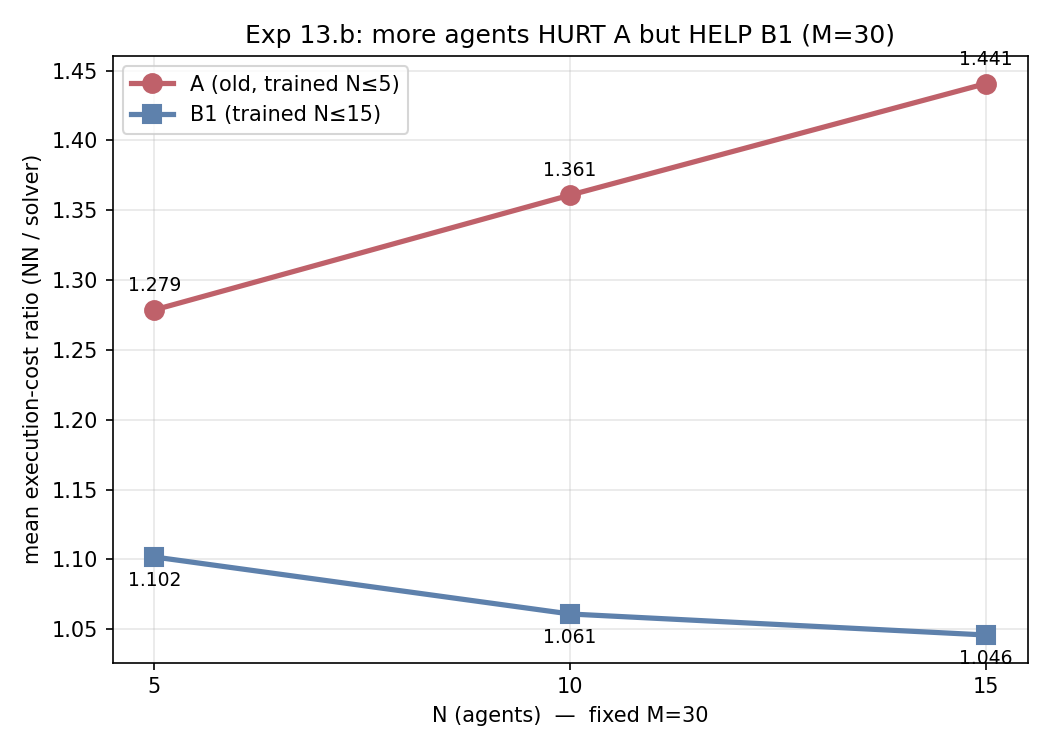
\includegraphics[width=\textwidth]{fig2_N_divergence_m30.png}\\[1pt]
  {\small (b) the scale-transfer scissors}
\end{minipage}
\caption{The two findings that set up the final study. \textbf{(a)} Goal-to-goal distances lift
full-assignment accuracy by 14 to 18 points at every agent count, the dominant design decision (D2).
\textbf{(b)} At $M{=}30$, adding agents hurts the small-scale-trained model but helps the map-trained
one, so generalization fails across problem scale, not across map geometry (D5).}
\label{fig:designfigs}
\end{figure}

\begin{findingbox}{Why this leads to the final study}
D5 showed that a model has to be trained on structured geometry in order to handle it, since the
entire advantage of map-based training over random-grid training came from the maze. If
geometry-specific structure matters that much, the natural next question is whether a dedicated
model per map outperforms one generalist serving all four. That is what Section~\ref{sec:final}
tests.
\end{findingbox}

% ═════════════════════════════════════════════════════════════════════════════
\section{Final Study: Scale Limits and Specialists versus a Generalist}
\label{sec:final}
% ═════════════════════════════════════════════════════════════════════════════

\subsection{Research questions}

\begin{enumerate}[label=\textbf{RQ\arabic*.}]
  \item How far can $N$ and $M$ grow before the exact solver becomes impractical, on the order of a
        minute per instance, and what does that imply for what can be labeled and measured?
  \item For each model role, which training distribution works better: many instances at regular
        size, or fewer instances at large size?
  \item Do per-map specialists outperform a single generalist, in quality and in wall-time, by
        enough to justify routing an instance to a map-specific model?
\end{enumerate}

\subsection{Design}

\textbf{The scale wall.} We sweep $N$ and $M$ on each map until the solver's mean wall-time
approaches 60 seconds. This bounds the study in three ways that should not be conflated. The
labeling ceiling is the largest $(N,M)$ at which the solver can still produce training labels in
acceptable time, which bounds what the large-instance dataset can contain. The evaluation ceiling is
the largest $(N,M)$ at which a solver baseline exists at all; past that point the cost ratio has no
denominator and cannot be computed. Beyond both, only solver-independent quantities remain
measurable.

\textbf{The model matrix.} Five roles, namely one generalist trained on all four maps and four
specialists trained on \texttt{empty}, \texttt{random}, \texttt{maze} and \texttt{room}
respectively, are each trained on two datasets: (A) many regular-size instances, and (B) fewer
large instances reaching toward the scale wall. This gives ten models, all h128/L6.

\textbf{Why only the smaller architecture.} We fix the network to h128/L6 because it beat the larger
h256/L8 in-distribution on every aggregate metric, with a $1.048$ versus $1.052$ execution-cost
ratio and $0.433$ versus $0.402$ exact match, while running roughly 20\% faster. The extra
$2.5\times$ in parameters bought no accuracy, and the larger model reached its validation optimum
early and then overfitted. The ranking does reverse far out of distribution, where the larger model
extrapolates better, but dataset~B places the large-instance regime inside the training distribution
by construction, so the in-distribution verdict is the applicable one.

\begin{TODO}{TEXT --- 1--2 sentences}
Replace the justification above if the actual reason for restricting to the smaller model differed.
The text reconstructs the rationale from the earlier h128-vs-h256 comparison; confirm it, or
substitute the real reasoning.
\end{TODO}

\textbf{Protocol.} All models see identical instances for a given (map, $N$, $M$) cell, which allows
paired comparison. The dataset choice for RQ2 is made on validation data, and the
specialist-versus-generalist comparison for RQ3 is reported on held-out test data, so the selection
step cannot inflate the final result. The generalist is scored per map and not pooled. Without
that, a uniformly mediocre generalist would be indistinguishable from one that is strong on three
maps and weak on the fourth.

\begin{TODO}{TABLE --- T2, the model inventory}
Ten rows: model id, role, training map(s), dataset (A/B), $N$ and $M$ ranges, samples per
configuration and in total, epochs, learning rate, batch size, gradient clipping, seeds, parameter
count, best validation loss and epoch, training wall-time. Note any model that hit its wall-clock
limit before finishing its epoch budget, since a wall-limited model must not be presented as a
converged one. \emph{Source: \texttt{model\_inventory.csv} (data request \S6.6).}
\end{TODO}

\subsection{Results}

\begin{TODO}{FIGURE + TEXT --- R1, the solver scale wall}
\emph{Figure:} exact-solver wall-time against problem size, one line per map, horizontal marker at
60\,s, log scale on time. \emph{Text ($\sim$100 words):} where the wall falls on each map, whether it
is driven by $N$ or $M$, and the three ceilings stated numerically.
\emph{Source: \texttt{solver\_scale\_wall.csv} (data request \S3).}
\end{TODO}

\begin{TODO}{TABLE + FIGURE + TEXT --- R2, dataset selection (RQ2)}
Five head-to-heads, one per role, each between its dataset-A and dataset-B model on a common
$(N,M)$ grid spanning both regimes. \emph{Figure:} cost ratio against problem size, one line per
dataset, showing where the curves cross. \emph{Table:} winner per role with the margin.
\emph{Text ($\sim$150 words):} whether the crossover is consistent across maps, and whether
many-small or few-large is the better use of a fixed labeling budget.
\emph{Source: \texttt{stage1\_dataset\_selection/} (data request \S4).}
\end{TODO}

\begin{TODO}{TABLE + FIGURE + TEXT --- R3, specialists versus the generalist (RQ3)}
The five selected models on all four maps. \emph{Table:} per map, specialist and generalist side by
side on execution-cost ratio, exact match, mean diff, per-goal and full-assignment accuracy, and mean
wall-time. \emph{Figure:} grouped bars per map, specialist against generalist, on cost ratio and on
speed. \emph{Text ($\sim$200 words):} whether the specialist advantage is real, whether it is uniform
across maps or concentrated on the structured ones (the D5 prediction), and whether it holds on
timing as well as quality. \emph{Source: \texttt{stage2\_expert\_vs\_general/} (data request \S5).}
\end{TODO}

\begin{TODO}{TABLE + TEXT --- R4, the cost of misrouting}
The full $5\times4$ matrix of every model on every map. The diagonal answers whether specialists are
better, and the off-diagonal answers what it costs when a router picks wrong.
\emph{Text ($\sim$120 words):} expected gain under a perfect router, the misrouting penalty, and
therefore how confident map identification has to be for routing to pay.
\emph{Source: \texttt{stage2\_expert\_vs\_general/} off-diagonal cells.}
\end{TODO}

\subsection{Hypotheses}

These predictions are recorded before the results are available, so that they can be confirmed or
refuted rather than rationalized afterward.

On RQ2, we expect dataset~A to win at small $(N,M)$ and dataset~B at large $(N,M)$, with a crossover
somewhere between, since each dataset places its own regime in-distribution. The interesting
quantity is not which one wins overall but where the crossover sits, because that determines how a
fixed labeling budget should be spent.

On RQ3, we expect the specialist advantage to be largest on \texttt{maze} and smallest on
\texttt{empty} and \texttt{random}, following D5. Training data mattered only for structured
geometry, so specialization should pay only where there is structure to specialize on. If instead
the specialists win uniformly across all four maps, the explanation would be capacity, with one
network split across four distributions, rather than geometry. That would be a more interesting
result than the one we predict.

On timing, we expect specialists and generalist to be indistinguishable, since the architecture is
identical and a forward pass costs the same either way. Any measured difference should be attributed
to the environment rather than the model, and one that survives scrutiny would be worth
investigating.

\begin{TODO}{TEXT --- $\sim$150 words}
After the results land, add a short verdict subsection: which hypotheses held, which failed, and what
the failures imply. Keep the predictions above unchanged, since a refuted prediction that is honestly
reported is worth more than one quietly edited to match.
\end{TODO}

% ═════════════════════════════════════════════════════════════════════════════
\section{Discussion}
% ═════════════════════════════════════════════════════════════════════════════

\textbf{When the learned allocator is the right choice.} It replaces the allocation step only, so it
pays off where allocation dominates and where many instances have to be solved. At large $N$ and
$M$, LKH's TSP grows expensive while the forward pass stays close to flat, which yields
5.9--9.4$\times$ end-to-end speedup at roughly 20\% above optimal cost. Under batched,
high-throughput use, allocation-only inference is orders of magnitude faster than the solver. On
unstructured geometry, even cheap random-grid training transfers, so no map-specific data collection
is needed. The opposite cases are equally clear. On small instances the exact solver already answers
in milliseconds and CBS dominates both pipelines, leaving nothing to save. Where exactness is
contractually required, an approximate allocator is inadmissible whatever its speed. And on
structured maps the network has to have trained on that structure, so an unseen structured
environment is a poor fit.

\textbf{Limitations.} Goal-visit ordering is a separate classical step in our pipeline. Exhaustive
enumeration is optimal but costs $O(k!)$, and it becomes the pipeline bottleneck at seven or eight
goals per agent, where the allocation itself is sub-millisecond but the step around it is not.
Beyond eight goals we fall back to nearest-neighbor with 2-opt, which is fast but no longer
guaranteed optimal. At that point some of the gap to the solver comes from our ordering instead of
our allocation, so the attribution is no longer clean, and a learned ordering head would remove both
problems at once. CBS execution cost is
not differentiable, so training optimizes an imitation proxy and not the objective actually being
measured. Imitation also caps quality at the teacher's level, meaning the network can match the exact
solver but never beat it. Finally, the evaluation rests on one $32\times32$ benchmark family under
basic, deterministic MAPF. Orientation, action delays, and larger or non-grid environments are
untested.

% ═════════════════════════════════════════════════════════════════════════════
\section{Conclusion}
% ═════════════════════════════════════════════════════════════════════════════

A compact transformer reading two distance matrices reproduces an exact solver's goal allocation
closely enough that the resulting collision-free plans cost 2\% more than optimal on average
in-distribution, with a single set of weights serving any number of agents and goals. The decisive
design choice turned out to be representation, not architecture or scale, since goal-to-goal
distances were worth more than every other improvement combined. The model generalizes across map
geometry but not across problem scale, and its speed advantage appears in exactly the regimes where
the exact solver's does not, at scale and in batch.

\begin{TODO}{TEXT --- 2--3 sentences}
Add the final study's conclusion: whether map specialists beat the generalist, whether routing is
justified, and which training distribution proved the better use of a labeling budget.
\end{TODO}

\textbf{Future work.} The solver's true tour cost is already computed during data generation and then
discarded. Storing it would enable a tour-aware loss term
$\sum_{j,k}\left(\sum_i P_{ij}P_{ik}\right)G_{jk}$ that directly penalizes splitting adjacent goals,
targeting the failure mode that dominates at high $M$. A learned goal-ordering head would remove the
last classical bottleneck. Approximate conflict penalties or policy-gradient signals could push
training toward the true MAPF objective instead of the imitation proxy.

\subsection*{Acknowledgements}

The RobustMCPF solver, the exact LKH and CBS pipeline used here for ground truth and as the
comparison baseline, is the work of Yehonatan Kidushim, Avraham Natan, Roni Stern and Meir Kalech,
and is not a contribution of this project. We thank the authors for permission to use it.

\begin{TODO}{TEXT --- verify before submission}
The references below are standard works, but their venues, years and page numbers have not been
checked against the originals. Verify each one. Related work (Section~2.4) is deliberately one
paragraph; expand it into a standalone section if the grader expects a fuller treatment.
\end{TODO}

% ═════════════════════════════════════════════════════════════════════════════
{\footnotesize
\begin{thebibliography}{99}
\setlength{\itemsep}{0pt}
\bibitem{robustmcpf} Y.~Kidushim, A.~Natan, R.~Stern, and M.~Kalech. Robust Multiagent Combinatorial
  Path Finding. \emph{AAAI}, 2026.
\bibitem{cbs} G.~Sharon, R.~Stern, A.~Felner, and N.~Sturtevant. Conflict-based search for optimal
  multi-agent pathfinding. \emph{Artificial Intelligence}, 219:40--66, 2015.
\bibitem{lkh} K.~Helsgaun. An effective implementation of the Lin--Kernighan traveling salesman
  heuristic. \emph{European Journal of Operational Research}, 126(1):106--130, 2000.
\bibitem{stern} R.~Stern et al. Multi-agent pathfinding: Definitions, variants, and benchmarks.
  \emph{Symposium on Combinatorial Search (SoCS)}, 2019.
\bibitem{sturtevant} N.~Sturtevant. Benchmarks for grid-based pathfinding. \emph{IEEE Transactions
  on Computational Intelligence and AI in Games}, 4(2):144--148, 2012.
\bibitem{ma_koenig} H.~Ma and S.~Koenig. Optimal target assignment and path finding for teams of
  agents. \emph{AAMAS}, 2016.
\bibitem{kaduri} O.~Kaduri, E.~Boyarski, and R.~Stern. Algorithm selection for optimal multi-agent
  pathfinding. \emph{ICAPS}, 2020.
\bibitem{primal} G.~Sartoretti et al. PRIMAL: Pathfinding via reinforcement and imitation
  multi-agent learning. \emph{IEEE Robotics and Automation Letters}, 4(3):2378--2385, 2019.
\bibitem{pointernet} O.~Vinyals, M.~Fortunato, and N.~Jaitly. Pointer networks. \emph{NeurIPS}, 2015.
\bibitem{bello} I.~Bello, H.~Pham, Q.~V.~Le, M.~Norouzi, and S.~Bengio. Neural combinatorial
  optimization with reinforcement learning. \emph{ICLR Workshop}, 2017.
\bibitem{kool} W.~Kool, H.~van Hoof, and M.~Welling. Attention, learn to solve routing problems!
  \emph{ICLR}, 2019.
\bibitem{bengio} Y.~Bengio, A.~Lodi, and A.~Prouvost. Machine learning for combinatorial
  optimization: a methodological tour d'horizon. \emph{European Journal of Operational Research},
  290(2):405--421, 2021.
\end{thebibliography}
}

% ── The one deliberate page break: the appendix starts fresh so the body's
%    page count is unambiguous if the appendix is excluded from the limit. ────
\clearpage
% ═════════════════════════════════════════════════════════════════════════════
\appendix
\section{Appendix}
% ═════════════════════════════════════════════════════════════════════════════

\begin{TODO}{TABLE --- full per-configuration results}
Complete per-configuration tables for the final study: every (model, map, $N$, $M$) cell with cost
ratio, exact match, mean/max/std diff, infeasible and fallback rates, timings, and $n$. The body
carries only aggregates and figures. \emph{Source: aggregate files accompanying
\texttt{stage2\_expert\_vs\_general/}.}
\end{TODO}

\begin{TODO}{TABLE --- reproducibility}
Hyperparameters and seeds for all ten models, cluster node types used for timing, torch version, and
whether inference ran on CPU or GPU. Timing numbers are uninterpretable without this.
\end{TODO}

\begin{TODO}{FIGURE --- optional, training convergence}
Train and validation loss and per-goal accuracy against epoch for the ten models, with the
best-validation checkpoint marked. Worth including if the models show the same overfitting signature
as earlier runs, where validation loss turned upward well before the epoch budget ended and
best-validation checkpointing acted as implicit early stopping.
\emph{Source: \texttt{train\_logs/} (data request \S6.5).}
\end{TODO}

\begin{TODO}{TEXT --- raw data pointers}
Record where the per-instance CSVs live (\texttt{report/data/exp16/}), the column schema, and the
cluster job identifiers, matching the convention used for earlier experiments.
\end{TODO}

\end{document}
